\documentclass[a4paper]{article} 
\usepackage{tcolorbox}
\tcbuselibrary{skins}

\title{
\vspace{-3em}
\begin{tcolorbox}[colframe=white,opacityback=0]
\begin{tcolorbox}
\Huge\sffamily Vocabulary and Definitions
\end{tcolorbox}
\end{tcolorbox}
\vspace{-3em}
}

\date{}

\usepackage{background}
\SetBgScale{1}
\SetBgAngle{0}
\SetBgColor{grey}
\SetBgContents{\rule[0em]{4pt}{\textheight}}
\SetBgHshift{-2.3cm}
\SetBgVshift{0cm}

\usepackage{lipsum}% just to generate filler text for the example
\usepackage[margin=2cm]{geometry}

\usepackage{tikz}
\usepackage{tikzpagenodes}

\parindent=0pt

\usepackage{xparse}
\DeclareDocumentCommand\topic{ m m g g g g g}
{
\begin{tcolorbox}[sidebyside,sidebyside align=top,opacityframe=0,opacityback=0,opacitybacktitle=0, opacitytext=1,lefthand width=.3\textwidth]
\begin{tcolorbox}[colback=red!05,colframe=red!25,sidebyside align=top,width=\textwidth,before skip=0pt]
#1\end{tcolorbox}%
\tcblower
\begin{tcolorbox}[colback=blue!05,colframe=blue!10,width=\textwidth,before skip=0pt]
#2
\end{tcolorbox}
\IfNoValueF {#3}{
\begin{tcolorbox}[colback=blue!05,colframe=blue!10,width=\textwidth]
#3
\end{tcolorbox}
}
\IfNoValueF {#4}{
\begin{tcolorbox}[colback=blue!05,colframe=blue!10,width=\textwidth]
#4
\end{tcolorbox}
}
\IfNoValueF {#5}{
\begin{tcolorbox}[colback=blue!05,colframe=blue!10,width=\textwidth]
#5
\end{tcolorbox}
}
\IfNoValueF {#6}{
\begin{tcolorbox}[colback=blue!05,colframe=blue!10,width=\textwidth]
#6
\end{tcolorbox}
}
\IfNoValueF {#7}{
\begin{tcolorbox}[colback=blue!05,colframe=blue!10,width=\textwidth]
#7
\end{tcolorbox}
}
\end{tcolorbox}
}

\def\summary#1{
\begin{tikzpicture}[overlay,remember picture,inner sep=0pt, outer sep=0pt]
\node[anchor=south,yshift=-1ex] at (current page text area.south) {% 
\begin{minipage}{\textwidth}%%%%
\begin{tcolorbox}[colframe=white,opacityback=0]
\begin{tcolorbox}[enhanced,colframe=black,fonttitle=\large\bfseries\sffamily,sidebyside=true, nobeforeafter,before=\vfil,after=\vfil,colupper=black,sidebyside align=top, lefthand width=.95\textwidth,opacitybacktitle=1, opacitytext=1,
segmentation style={black!55,solid,opacity=0,line width=3pt},
title=Summary
]
#1
\end{tcolorbox}
\end{tcolorbox}
\end{minipage}
};
\end{tikzpicture}
}

\usepackage{graphicx}
\usepackage{physics}
\usepackage{amsmath}
\usepackage{tikz}
\usepackage{mathdots}
\usepackage{yhmath}
\usepackage{cancel}
\usepackage{color}
\usepackage{siunitx}
\usepackage{array}
\usepackage{multirow}
\usepackage{amssymb}
\usepackage{gensymb}
\usepackage{tabularx}
\usepackage{booktabs}
\usetikzlibrary{fadings}
\usetikzlibrary{patterns}
\usetikzlibrary{shadows.blur}
\usetikzlibrary{shapes}

\begin{document} 
\maketitle

\topic{Exigence}{The need or demand. Why is \underline{NOW} the time \& place for a message}%

\topic{Rhetoric}{The ability to discern the available means of persuasion in any given situation.}%

\topic{Visual Rhetoric}{``Writing with images'' Ex. documentaries, illustrations, advertisements, cartoons, etc.}%

\topic{Audience}{A group to whom a work is meant to be presented to. Must establish what the viewer's values or morals are in order to have an effective message}%

\topic{Text}{Products meant to be read}%

\topic{Context}{Parts of discourse that surround a word or passage}%

\topic{Rhetorical Triangle}{A way to conceptualize the relationship between elements of a text}%

\summary{\centering\tikzset{every picture/.style={line width=0.75pt}} %set default line width to 0.75pt        

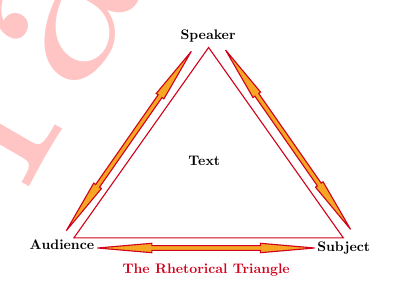
\begin{tikzpicture}[x=0.75pt,y=0.75pt,yscale=-.5,xscale=.5]
%uncomment if require: \path (0,374); %set diagram left start at 0, and has height of 374

%Shape: Triangle [id:dp3926678547967024] 
\draw  [color={rgb, 255:red, 208; green, 2; blue, 27 }  ,draw opacity=1 ][fill={rgb, 255:red, 255; green, 255; blue, 255 }  ,fill opacity=1 ] (326.32,82.68) -- (456.15,266.17) -- (196.49,266.17) -- cycle ;
%Left Right Arrow [id:dp19943991138135786] 
\draw  [color={rgb, 255:red, 208; green, 2; blue, 27 }  ,draw opacity=1 ][fill={rgb, 255:red, 245; green, 166; blue, 35 }  ,fill opacity=1 ] (219.28,275.9) -- (271.6,271.36) -- (271.6,273.63) -- (376.23,273.63) -- (376.23,271.36) -- (428.54,275.9) -- (376.23,280.43) -- (376.23,278.16) -- (271.6,278.16) -- (271.6,280.43) -- cycle ;
%Left Right Arrow [id:dp20777623482608543] 
\draw  [color={rgb, 255:red, 208; green, 2; blue, 27 }  ,draw opacity=1 ][fill={rgb, 255:red, 245; green, 166; blue, 35 }  ,fill opacity=1 ] (189.21,259.22) -- (215.64,213.39) -- (217.49,214.7) -- (277.73,128.29) -- (275.88,126.97) -- (309.69,86.39) -- (283.26,132.22) -- (281.41,130.91) -- (221.18,217.32) -- (223.02,218.64) -- cycle ;
%Left Right Arrow [id:dp7601860485249441] 
\draw  [color={rgb, 255:red, 208; green, 2; blue, 27 }  ,draw opacity=1 ][fill={rgb, 255:red, 245; green, 166; blue, 35 }  ,fill opacity=1 ] (463.11,257.92) -- (436.64,212.11) -- (434.82,213.41) -- (374.58,127) -- (376.41,125.7) -- (342.63,85.09) -- (369.09,130.9) -- (370.92,129.6) -- (431.16,216.02) -- (429.33,217.32) -- cycle ;


% Text Node
\draw (305.67,186.02) node [anchor=north west][inner sep=0.75pt]  [xscale=0.5,yscale=0.5] [align=left] {\textbf{Text}};
% Text Node
\draw (152.51,267.07) node [anchor=north west][inner sep=0.75pt]  [xscale=0.5,yscale=0.5] [align=left] {\textbf{Audience}};
% Text Node
\draw (429.75,268.37) node [anchor=north west][inner sep=0.75pt]  [xscale=0.5,yscale=0.5] [align=left] {\textbf{Subject}};
% Text Node
\draw (298.08,64.13) node [anchor=north west][inner sep=0.75pt]  [xscale=0.5,yscale=0.5] [align=left] {\textbf{Speaker}};
% Text Node
\draw (242.16,290.41) node [anchor=north west][inner sep=0.75pt]  [xscale=0.5,yscale=0.5] [align=left] {\textbf{\textcolor[rgb]{0.82,0.01,0.11}{The Rhetorical Triangle}}};


\end{tikzpicture}
}

\newpage

\topic{Occasion}{Specific circumstances surrounding the creation of a text}%

\topic{Purpose}{The goal an author intends to achieve}%

\topic{Speaker}{The author of the text}%

\topic{Persona}{The difference between the speaker on and off stage}%

\topic{Subject}{The topic of the text}%

\topic{Ethos}{Greek word for character. Expertise, knowledge, sincerity. Conveys shared values}%

\topic{Pathos}{Emotions, desires, hopes, fears, prejudices. Rests with connotations}%

\topic{Logos}{Clear rational ideas, backed with statistics, examples, or details. Logic}%

\topic{\textit{The King's Speech}}{Answer the questions}%

\topic{Question 1 $-$ How do you think King George VI felt during this speech?}{First and foremost, King George VI most likely feared for himself and his people. In addition to this, he probably felt powerful, as all of his citizens were listening to him at once. Also, he probably feels anxious and concerned about going into the war.}%

\topic{Question 2 $-$ What is the emotion behind this speech?}{Sorrow, courage, patriotic, powerful.}%

\topic{SPACECAT}{\begin{tabular}{r|l} S & peaker \\ P & urpose \\ A & udience \\ C & ontext \\ E & xigence \\ C & hoices \\ A & ppeals  \\ T & one  \\ \end{tabular}}%

    \topic{When thinking of the speaker\dots}{What are their beliefs and values? Do we trust them? Why? What do we know and not know about them? Is there meaning behind who wrote or said it?}%

    \topic{When thinking of the purpose\dots}{What is the speaker hoping to accomplish? What reaction are they trying to elicit, and how do they want us to behave? Think of the purpose as an infinitive: to + verb.}%

    \topic{When thinking of the audience\dots}{What did the speaker assume about their audience? How does that impact what they say and how they say it?}%

    \topic{When thinking of the context\dots}{What was going on in the world when this text was produced?}%

    \topic{When thinking of the exigence\dots}{What was the spark or catalyst that moved the speaker to act?}%

    \topic{When thinking of the choices\dots}{This is a category of all the little moves authors make to enrich their writing. Why does the writer make each choice?}%

    \topic{When thinking of the appeals\dots}{Appeals to the ethics or credibility, emotion, or logic or reason.}%

    \topic{When thinking of the tone\dots}{What is the speaker's attitude at different places throughout the text? How can you tell this is their attitude? Where does the tone shift in the piece?}%

    \topic{Examples: Spread vs Smear, Weep vs Cry vs Sob}{Connotation $-$ The certain feeling behind a word or phrase}%

    \topic{Diction}{A speaker's choice of words.}%

    \topic{Syntax}{How the words are arranged.}%

    \topic{Tone}{The speaker's attitude toward the subject as revealed by his or her choice of language.}%

    \topic{Mood}{The feeling created by the work.}%

    \topic{Metaphor}{A word or phrase that represents something other than the top meaning.}%

    \topic{Simile}{When two things are compared, usually using the phrases: \textit{like}, or \textit{as\dots as}.}%

    \topic{Personification}{When an inanimate object is given human attributes and characteristics.}%

    \topic{Hyperbole}{An obvious exaggeration.}%

    \topic{Parallelism}{Use of similar or identical syntaxes in different clauses or phrases.}%

    \topic{Juxtaposition}{When two things are placed side by side, usually to compare.}%

    \topic{Antithesis}{Synonymous with counterclaim.}%

    \topic{Compound Complex}{A sentence that uses the structure of both, a compound and a complex sentence.}%

    \topic{Periodic}{Something recurring in intervals.}%

    \topic{Cumulative}{Something that increases in size.}%

    \topic{Imperative}{When something is conveyed as necessary or urgent.}%

    \topic{Imagery}{The use of mental pictures or images.}%

    \topic{Oxymoron}{When two contradictory items are placed together.}%
 

%\topic{Here's another question to begin the new page.}{\lipsum[3]}%
%{\lipsum[4]}%
%{\lipsum[5]}%

%\summary{And another summary that will float to the bottom of the next page.}

\end{document}
